\documentclass[11pt]{article}
\usepackage{amsmath} 
\usepackage{amssymb}
\usepackage[margin=0.5in]{geometry}
\newcommand{\ds}{\displaystyle}
\usepackage{graphicx}
\usepackage{color}
\usepackage{booktabs}
\usepackage[oztex]{harpoon}
\usepackage{bbm}  

\begin{document}
	
\begin{center}\section*{MATH 316D W11}\end{center}
\subsection*{DD1 Individual Quiz}
\begin{enumerate}
	\item Match the terms with the definitions. (This is a matching question. The definitions are next to the term that it goes with. In the quiz, don't let them match up. Thank you!)
	\begin{enumerate}
		\item Equilibrium Solutions $\implies$ $x(t)$ is constant for all values of $t$. 
		\item Stable equilibrium $\implies$ every non-constant solution approaches the equilibrium. 
		\item Unstable equilibrium $\implies$ every non-constant solution flows away from the equilibrium. 
		\item Repelling Node $\implies$ the eigenvalues are positive and all solutions flow away from the equilibrium. 
		\item Attracting Node $\implies$ the eigenvalues are negative and all solutions approach the equilibrium.  
		\item Saddle Point $\implies$ the eigenvalues have opposite signs and some solutions are moving away while others are moving toward the equilibrium. 
	\end{enumerate}
	\item Let $A = \begin{bmatrix}
	-2&1\\0&-3
	\end{bmatrix}$. \\\\Then $\vec{x}' = A\vec{x}$ is best represented by 
	\begin{enumerate}
		\item $x_1' = -2x_1 + x_2$$\implies$ \textbf{This is the correct answer.} \\$x_2' = 0x_1-3x_2$ 
		\item $x_1' = 0x_1-3x_2$$\implies$ \textbf{Feedback: Make sure you have the correct rows.}\\$x_2' = -2x_1+x_2$
		\item $x_1' = x_1-2x_2$$\implies$ \textbf{Feedback: Check the columns of your matrix.}\\$x_2' = -3x_1+0x_2$
		\item $x_1' = 2x_1-x_2$$\implies$ \textbf{Feedback: Check the signs of your matrix.}\\$x_2' = 0x_1+3x_2$
	\end{enumerate}
	\item The eigenvalues for $A$ in problem 2 are:
	\begin{enumerate}
		\item both positive and real. $\implies$ \textbf{Feedback: Don't drop a negative.}
		\item both negative and real. $\implies$ \textbf{This is the correct answer.}
		\item opposite signs. $\implies$ \textbf{Feedback: Watch your signs.}
		\item one equals zero. $\implies$ \textbf{Feedback: Check your work once more.}
	\end{enumerate}
	\item Mark all that apply if the eigenvalues for matrix $A$ in $\vec{x}' = A\vec{x}$ are both positive real numbers.
	\begin{enumerate}
		\item $\vec{0}$ is a stable equilibrium. $\implies$ \textbf{Feedback: Check your definition.}
		\item $\vec{0}$ is an unstable equilibrium. $\implies$ \textbf{Feedback: Correct}
		\item $\vec{0}$ is a repelling node. $\implies$ \textbf{Feedback: Correct.}
		\item $\vec{0}$ is an attracting node. $\implies$ \textbf{Feedback: Check your definition.}
		\item $\vec{0}$ is a saddle point. $\implies$ \textbf{Feedback: Check your definition.}
	\end{enumerate}
	\item If a $2\times 2$ matrix $A$ has one eigenvalue equal to zero while the other is real, then $\vec{x}' = A\vec{x}$ has: (Mark all that apply)
	\begin{enumerate}
		\item more than one equilibrium solution. $\implies$ \textbf{Feedback: Correct.}
		\item exactly one equilibrium solution. $\implies$ \textbf{Feedback: Check your definition.}
		\item exactly one straight line solution. $\implies$ \textbf{Feedback: Check your definition.}
		\item more than one straight line solution. $\implies$ \textbf{Feedback: Correct.}
	\end{enumerate}
\newpage
	\item Use the Wronksian Theorem to determine the linearity of $\vec{v_1} = [e^{-t} \:\: -e^{-t} \:\: e^{-t}]^T$, $\vec{v_2} = [3e^{2t} \:\: e^{2t}\:\: -2e^{2t}]^T$, and $\vec{v_3} = [e^{5t} \:\: e^{5t}\:\:e^{5t}]^T$. Mark the true statement. 
	\begin{enumerate}
		\item The Wronksian is $10e^{6t}$ and thus $v_1$, $v_2$, and $v_3$ are linearly independent. $\implies$ \textbf{Feedback: Correct.}
		\item The Wronksian is $0$ and thus $v_1$, $v_2$, and $v_3$ are linearly independent. $\implies$ \textbf{Feedback: Check your determinate.}
		\item The Wronksian is $10e^{6t}$ and thus $v_1$, $v_2$, and $v_3$ are linearly dependent. $\implies$ \textbf{Feedback: Check the Wronksian.}
		\item The Wronksian is $0$ and thus $v_1$, $v_2$, and $v_3$ are linearly dependent. $\implies$ \textbf{Feedback: Check your determinate.}
	\end{enumerate}
\end{enumerate}
\subsection*{DD2 Group Quiz}
\begin{enumerate}
	\item Classify the stability of the orgin as an equilibrium for $\vec{x}' = A\vec{x}$ if $p(\lambda)$ is the characteristic equation determined by det$(A-\lambda I)$.\\$p(\lambda) = \lambda^2 + \lambda+1$.
	\begin{enumerate}
		\item Unstable repelling node
		\item Unstable saddle
		\item Stable center
		\item Stable spiral sink $\implies$ \textbf{Correct}
		\item Unstable spiral source
	\end{enumerate}
	\item Classify the stability of the orgin as an equilibrium for $\vec{x}' = A\vec{x}$ if $p(\lambda)$ is the characteristic equation determined by det$(A-\lambda I)$.\\$p(\lambda) = \lambda^2 -4$.
	\begin{enumerate}
		\item Unstable repelling node
		\item Unstable saddle $\implies$ \textbf{Correct}
		\item Stable center
		\item Stable spiral sink 
		\item Unstable spiral source
	\end{enumerate}
	\textbf{Instructions:} For questions 3 - 6, let $A = \begin{bmatrix}
	0&-2\\2&0
	\end{bmatrix}$, with initial values of $x_1(0) = 1$ and $x_2(0) = -1$.
	\item Determine the solution to $\vec{x}' = A\vec{x}$.
	\begin{enumerate}
		\item $\vec{x}(t) = c_1e^{3t}\begin{bmatrix}1\\0 \end{bmatrix} + c_2e^{-3t}\begin{bmatrix}0\\1 \end{bmatrix}$
		\item $\vec{x}(t) = c_1e^{3it}\begin{bmatrix}1\\0 \end{bmatrix} + c_2e^{-3it}\begin{bmatrix}0\\1 \end{bmatrix}$
		\item $\vec{x}(t) = c_1\begin{bmatrix}\cos(2t)\\\sin(2t)\end{bmatrix} + c_2e^{-3t}\begin{bmatrix}-\cos(2t)\\-\sin(2t)\end{bmatrix}$
		\item $\vec{x}(t) = c_1\begin{bmatrix}-\sin(2t)\\\cos(2t)\end{bmatrix} + c_2\begin{bmatrix}\cos(2t)\\\sin(2t)\end{bmatrix}$ $\implies$ \textbf{Correct}
		\item None of the above. 
	\end{enumerate}
\newpage
	\item Now, consider the IVP $\vec{x}' = A\vec{x}$ where $x_1(0) = 1$ and $x_2(0) = -1$. Solve. 
	\begin{enumerate}
		\item $\vec{x}(t) = e^{3t}\begin{bmatrix}1\\0 \end{bmatrix} -e^{-3t}\begin{bmatrix}0\\1 \end{bmatrix}$
		\item $\vec{x}(t) = -1\begin{bmatrix}-\sin(2t)\\\cos(2t)\end{bmatrix} + \begin{bmatrix}\cos(2t)\\\sin(2t)\end{bmatrix}$  $\implies$ \textbf{Correct}
		\item $\vec{x}(t) = -1\begin{bmatrix}\cos(2t)\\\sin(2t)\end{bmatrix} + e^{-3t}\begin{bmatrix}-\cos(2t)\\-\sin(2t)\end{bmatrix}$
		\item $\vec{x}(t) = -2\begin{bmatrix}-\sin(2t)\\\cos(2t)\end{bmatrix} + 2\begin{bmatrix}\cos(2t)\\\sin(2t)\end{bmatrix}$ 
		\item None of the above.
	\end{enumerate}
	\item Classify the stability of the equilibrium solution $\begin{bmatrix}0\\0 \end{bmatrix}$.
	\begin{enumerate}
		\item Unstable repelling node
		\item Stable attracting node
		\item Unstable spiral source
		\item Stable center $\implies$ \textbf{Correct}
		\item Stable spiral sink
	\end{enumerate}
	\item How many straight line solutions?
	\begin{enumerate}
		\item None $\implies$ \textbf{Correct}
		\item One
		\item Two
		\item Infinite
		\item Cannot be determined
	\end{enumerate}
\end{enumerate}

\subsection*{DD3 Weekly Quiz}
	\textbf{\textcolor{red}{This quiz needs to be completely redone so please delete all the current questions in i-Learn and replace them with the following, thank you.}}
		
	\begin{enumerate}
		\item ``In a system of three tanks of saltwater interconnected with pipes of inflow and outflow to and from each, the following information is given.

			\begin{table}[htbp]\centering
  				\begin{tabular}{|l|l|l|l|}
    					\hline
          					& Tank A & Tank B & Tank C \\
    					\hline
   						 Tank volume & 400 liters & 800 liters & 500 liters \\
   					 \hline
  					  	Rate of inflow
						to tank & 5 L/min. & 10 L/min. & 5 L/min. \\
    					\hline
    						Concentration of 
						salt in inflow & 25 g/L & 15 g/L & 40 g/L \\
    					\hline
    						Rate of drain outflow & 4 L/min. & 7 L/min. & 9 L/min. \\
   					\hline
						Rates of outflows 
						to other tanks & to B: 6 L/min. & to C: 5 L/min. & to A: 4 L/min. \\
    					\hline
    						Rates of outflows 
						to other tanks & to C: 4 L/min. & to A: 5 L/min. & to B: 1 L/min. \\
    					\hline
    				\end{tabular}
			\end{table}
			
			Assume that, initially, there is a concentration of $10$ g/L of salt in each of the three tanks. Set up an IVP of the system of tanks using the information given, then choose the answer that best represents your work."
				\begin{enumerate}
					\item \(\begin{bmatrix}
							A' \\ B' \\ C'
						 \end{bmatrix}=\begin{bmatrix}
										-7/200 & 1/160 & 1/125 \\
										3/200 & -17/800 & 1/500 \\
										1/100 & 1/160 & -7/250 \\
						 			\end{bmatrix}												\begin{bmatrix}
										A \\ B \\ C
									\end{bmatrix}\),\											\(\begin{bmatrix}
										A(0) \\ B(0) \\ C(0)
									\end{bmatrix}=												\begin{bmatrix}
										4000 \\ 8000 \\ 5000
									\end{bmatrix}\)			
					\item \(\begin{bmatrix}
							A' \\ B' \\ C'
						 \end{bmatrix}=\begin{bmatrix}
										-7/200 & 1/160 & 1/125 \\
										3/200 & -17/800 & 1/500 \\
										1/100 & 1/160 & -7/250 \\
						 			\end{bmatrix}												\begin{bmatrix}
										A \\ B \\ C
									\end{bmatrix}+													\begin{bmatrix}
											125 \\ 150 \\ 200													\end{bmatrix}\),\ 						\(\begin{bmatrix}
										A(0) \\ B(0) \\ C(0)
									\end{bmatrix}=												\begin{bmatrix}
										10 \\ 10 \\ 10
									\end{bmatrix}\)	

					
					\item \(\begin{bmatrix}
							A' \\ B' \\ C'
						 \end{bmatrix}=\begin{bmatrix}
										-7/200 & 1/160 & 1/125 \\
										3/200 & -17/800 & 1/500 \\
										1/100 & 1/160 & -7/250 \\
						 			\end{bmatrix}												\begin{bmatrix}
										A \\ B \\ C
									\end{bmatrix}+													\begin{bmatrix}
											125 \\ 150 \\ 200													\end{bmatrix}\),\ \(\begin{bmatrix}
										A(0) \\ B(0) \\ C(0)
									\end{bmatrix}=												\begin{bmatrix}
										4000 \\ 8000 \\ 5000
									\end{bmatrix}\)	 $\implies$ \textbf{Correct}
					
					\item \(\begin{bmatrix}
							A' \\ B' \\ C'
						 \end{bmatrix}=\begin{bmatrix}
										-7/200 & 1/160 & 1/125 & 125 \\
										3/200 & -17/800 & 1/500 & 150 \\
										1/100 & 1/160 & -7/250 & 200 \\
						 			\end{bmatrix}												\begin{bmatrix}
										A \\ B \\ C
									\end{bmatrix}\),\ \(\begin{bmatrix}
										A(0) \\ B(0) \\ C(0)
									\end{bmatrix}=												\begin{bmatrix}
										10 \\ 10 \\ 10
									\end{bmatrix}\)																	
					\item None of the above.
				\end{enumerate}

		\item ``Let us consider a system of two masses attached to two springs in parallel, where the mass $m_1$ is attached to the spring with spring constant $k_1$, and $m_2$ to the spring with constant $k_2$.  Assuming that the surface they are on is frictionless the equations that govern the systems motion is:
			
			
			\begin{centering}
				\(x_{1}''=-\dfrac{k_1}{m_1}x_1+\dfrac{k_2}{m_1}\left(x_2-x_1\right)\) 
				
				\(x_{2}''=-\dfrac{k_2}{m_2}\left(x_2-x_1\right)\).
			
			\end{centering}
			
			Suppose that $k_1$=2, $m_1$=1, $k_2$=4 and $m_2$=.5 . Using these constants and the following substitutions: $y_1=x_1$, $y_2=y_{1}'=x_{1}'$, $y_3=x_2$, $y_4=y_3=x_{2}'$, convert the system of two second-order equations to a system of the form $\overrightharp{y}'=\mathbbmss{A}\overrightharp{y}$."
			
				\begin{enumerate}
					\item \(\begin{bmatrix} y_{2}' \\ y_{4}' \end{bmatrix}=\begin{bmatrix} 2 & -4 \\ -8 & 8 \end{bmatrix} \begin{bmatrix} y_1 \\ y_3 \end{bmatrix}\)
					
					\item \(\begin{bmatrix} y_{1}' \\ y_{2}' \end{bmatrix}=\begin{bmatrix} -6 & 4 \\ 8 & -8 \end{bmatrix} \begin{bmatrix} y_1 \\ y_2 \end{bmatrix}\)
					
					\item \(\begin{bmatrix} y_{2}' \\ y_{4}' \end{bmatrix}=\begin{bmatrix} -6 & 4 \\ 8 & -8 \end{bmatrix} \begin{bmatrix} y_1 \\ y_3 \end{bmatrix}\) $\implies$ \textbf{Correct}
					
					\item None of the above.
				\end{enumerate}
				
		\item ``Suppose we have an RLC circuit that has an inductor of $L$=1 H, resistor of $R$=16 $\Omega$, and capacitor of $C$=.01 F. Assume that $I(0)$=100 A and $I'(0)$=0, and that the system is provided a voltage source of $E(t)=100\sin{10\, t}$."
		
		``State a second-order IVP whose solution is $I(t)$, the current in the circuit at time $t$."
			\begin{enumerate}
				\item \(I''(t)+16\,I'(t)+100\,I(t)=1000\cos{10\, t};\ I'(0)=0,\, I(0)=100\) $\implies$ \textbf{Correct}
				
				\item \(I''(t)+16\,I'(t)+.01\,I(t)=1000\cos{10\, t};\ I'(0)=100,\, I(0)=0\)
				
				\item \(I'(t)+16\,I(t)+100\,Q(t)=100\sin{10\,t};\ I'(0)=0,\, I(0)=100\)
				
				\item None of the above.
			\end{enumerate}
		
		\item ``Using your answer from the previous problem, create a system of first-order IVPs using a standard substitution and in the standard form \(\overrightharp{x}'=\mathbbmss{A}\overrightharp{x}\)."
		
			\begin{enumerate}
				\item \(\begin{bmatrix} x_{1}'(t) \\ x_{2}'(t) \end{bmatrix}=\begin{bmatrix} 0 & 1 \\ -100 & -16 \end{bmatrix}\begin{bmatrix} x_{1}(t) \\ x_{2}(t) \end{bmatrix}+\begin{bmatrix} 0 \\ 1000\cos{10\,t} \end{bmatrix};\ \begin{bmatrix} x_{1}(0) \\ x_{2}(0) \end{bmatrix}=\begin{bmatrix} 100 \\ 0 \end{bmatrix}\)
 $\implies$ \textbf{Correct}
				
				\item \(\begin{bmatrix} x_{1}'(t) \\ x_{2}'(t) \end{bmatrix}=\begin{bmatrix} 0 & 1 \\ -100 & -.01 \end{bmatrix}\begin{bmatrix} x_{1}(t) \\ x_{2}(t) \end{bmatrix}+\begin{bmatrix} 0 \\ 1000\cos{10\,t} \end{bmatrix};\ \begin{bmatrix} x_{1}(0) \\ x_{2}(0) \end{bmatrix}=\begin{bmatrix} 0 \\ 100 \end{bmatrix}\)

				
				\item \(\begin{bmatrix} x_{1}'(t) \\ x_{2}'(t) \end{bmatrix}=\begin{bmatrix} 0 & 1 \\ -100 & -16 \end{bmatrix}\begin{bmatrix} x_{1}(t) \\ x_{2}(t) \end{bmatrix}+\begin{bmatrix} 0 \\ 100\sin{10\,t} \end{bmatrix};\ \begin{bmatrix} x_{1}(0) \\ x_{2}(0) \end{bmatrix}=\begin{bmatrix} 100 \\ 0 \end{bmatrix}\)
				
				\item None of the above.
			\end{enumerate}
		
		\item ``From your model, as defined in question four, state what the eigenpairs are."
			\begin{enumerate}
				\item \(\left\{\lambda_{1}=0, \overrightharp{v}_1=\begin{bmatrix} 0 \\ 0 \end{bmatrix}\right \}\) and \(\left\{\lambda_{2}=-16, \overrightharp{v}_2=\begin{bmatrix} 0 \\ 0 \end{bmatrix}\right \}\)
				
				\item \(\left\{\lambda_{1}=-8+6i, \overrightharp{v}_1=\begin{bmatrix} -(4-3i) \\ 50 \end{bmatrix}\right \}\) and \(\left\{\lambda_{2}=-8-6i, \overrightharp{v}_2=\begin{bmatrix} -(4+3i) \\ 50 \end{bmatrix}\right \}\)
				
				\item \(\left\{\lambda_{1}=-.005+10i, \overrightharp{v}_1=\begin{bmatrix} -(5\cdot 10^{-5}+.1i) \\ 1 \end{bmatrix}\right \}\) and \(\left\{\lambda_{2}=-.005-10i, \overrightharp{v}_2=\begin{bmatrix} -(5\cdot 10^{-5}-.1i) \\ 1 \end{bmatrix}\right \}\)
				
				\item \(\left\{\lambda_{1}=-8+6i, \overrightharp{v}_1=\begin{bmatrix} -(4+3i) \\ 50 \end{bmatrix}\right \}\) and \(\left\{\lambda_{2}=-8-6i, \overrightharp{v}_2=\begin{bmatrix} -(4-3i) \\ 50 \end{bmatrix}\right \}\) $\implies$ \textbf{Correct}
			\end{enumerate}
			
		\item ``Which of the following graphs represents the direction field of the eigenpair from the system you defined in problem four?"
		
			\begin{enumerate}
				\item \begin{figure}[h!]
					\graphicspath{{/Users/tylertrogden/Desktop/}}
					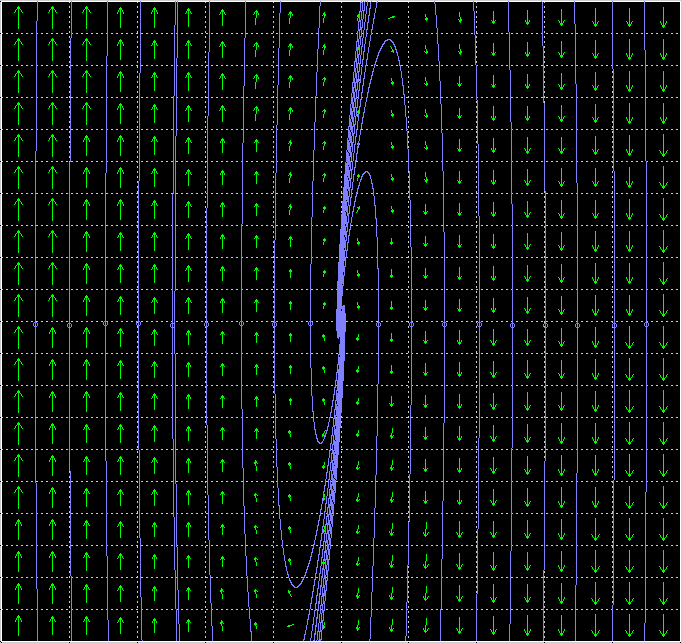
\includegraphics[height=3cm,width=8cm]{W11_WQ_Q6(a)} 
					\end{figure}

				
				\item \begin{figure}[h!]
					\graphicspath{{/Users/tylertrogden/Desktop/}}
					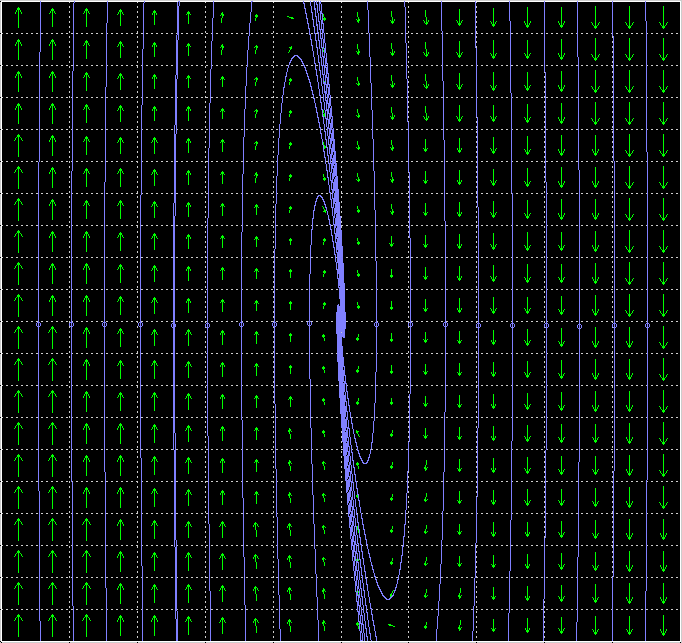
\includegraphics[height=3cm,width=8cm]{W11_WQ_Q6(b)} $\implies$ \textbf{Correct}
					\end{figure}

				
				\item \begin{figure}[h!]
					\graphicspath{{/Users/tylertrogden/Desktop/}}
					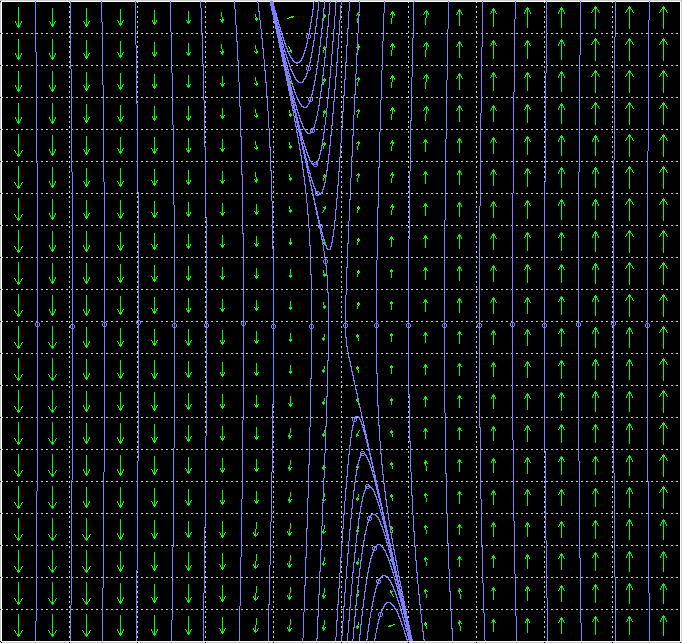
\includegraphics[height=3cm,width=8cm]{W11_WQ_Q6(c)} 
					\end{figure}

				
				\item \begin{figure}[h!]
					\graphicspath{{/Users/tylertrogden/Desktop/}}
					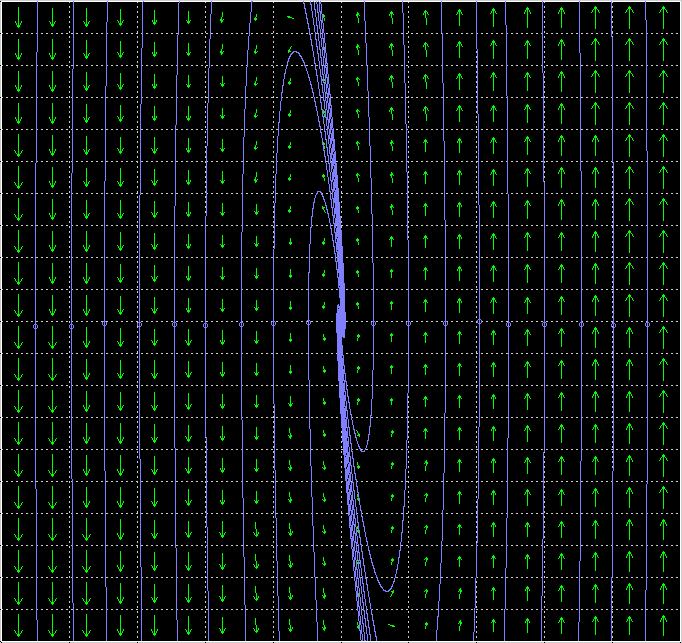
\includegraphics[height=3cm,width=8cm]{W11_WQ_Q6(d)} 
					\end{figure}

			\end{enumerate}

		\item ``Solve the system that you defined in problem four to determine the current $I(t)$ at time $t$. You may use Mathematica to help find the solution but \textcolor{red}{you may not use} the commands \texttt{DSolve} or \texttt{NDSolve}."
		
			\begin{enumerate}
				\item \(\overrightharp{x}_{g}(t)=-\left(\dfrac{5}{8}-\dfrac{95i}{6}\right)e^{(-8+6i)t} \begin{bmatrix} -(4+3i) \\ 50 \end{bmatrix}-\left(\dfrac{5}{8}+\dfrac{95i}{6}\right)e^{-(8+6i)t} \begin{bmatrix} -(4-3i) \\ 50 \end{bmatrix}+\begin{bmatrix} -\frac{5}{8}\cos{10\,t} \\[.5em] \frac{25}{4}\sin{10\,t} \end{bmatrix}\)
				\item \(\overrightharp{x}_{g}(t)=-\left(\dfrac{5}{8}-\dfrac{95i}{6}\right)e^{(-8+6i)t} \begin{bmatrix} -(4+3i) \\ 50 \end{bmatrix}-\left(\dfrac{5}{8}+\dfrac{95i}{6}\right)e^{-(8+6i)t} \begin{bmatrix} -(4-3i) \\ 50 \end{bmatrix}+\begin{bmatrix} \frac{25}{4}\sin{10\,t} \\[.5em] \frac{125}{2}\cos{10\,t} \end{bmatrix}\) $\implies$ \textbf{Correct}
				
				\item \(\overrightharp{x}_{g}(t)=-\left(\dfrac{5}{8}-\dfrac{95i}{6}\right)e^{(-8+6i)t} \begin{bmatrix} -(4-3i) \\ 50 \end{bmatrix}-\left(\dfrac{5}{8}+\dfrac{95i}{6}\right)e^{-(8+6i)t} \begin{bmatrix} -(4+3i) \\ 50 \end{bmatrix}+\begin{bmatrix} \frac{25}{4}\sin{10\,t} \\[.5em] \frac{125}{2}\cos{10\,t} \end{bmatrix}\)
				
				\item None of the above.
			\end{enumerate}
				
		\item \textbf{(Essay Question)} ``Consider a system of two tanks that are connected in such a way that each of the tanks has an independent inflow that delivers salt solution to it, each has an independent outflow (i.e. drain), and each tank is connected to the other with an outflow and an inflow. The relevant information is as follows:
		
				\begin{table}[htbp]\centering
  				\begin{tabular}{|l|l|l|}
    					\hline
          					& Tank A & Tank B \\
    					\hline
   						 Tank volume & 100 liters & 200 liters \\
   					 \hline
  					  	Rate of inflow
						to tank & 5 L/min. & 9 L/min. \\
    					\hline
    						Concentration of 
						salt in inflow & 7 g/L & 3 g/L \\
    					\hline
    						Rate of drain outflow & 4 L/min. & 10 L/min. \\
   					\hline
						Rates of outflows 
						to other tanks & to B: 3 L/min. & to A: 2 L/min. \\
    					\hline
    					
    				\end{tabular}
			\end{table}
		With Tank A initially having $20$ g of salt present in solution, and Tank B having $75$ g of salt present in solution."
		
		``Set up and solve an IVP whose solution will determine the amount of salt in each tank at time $t$. You may use Mathematica to help you solve the IVP, but \textcolor{red}{you may not use} \texttt{DSolve} or \texttt{NDSolve} to help you find the solution in Mathematica. Once you have found the answer please upload all your work here including your Mathematica notebook or screen shot." The answer should be along the lines of: 1) the IVP set up as \(\begin{bmatrix}A'(t) \\ B'(t) \end{bmatrix}=\begin{bmatrix} -\frac{7}{100} & \frac{1}{100} \\[.5em] \frac{3}{100} & -\frac{3}{50} \end{bmatrix}\begin{bmatrix}A(t) \\ B(t) \end{bmatrix}+\begin{bmatrix} 35 \\ 27 \end{bmatrix}\)	with \(\begin{bmatrix} A(0) \\ B(0) \end{bmatrix}=\begin{bmatrix} 20 \\ 75 \end{bmatrix}\) and 2) the answer		
		
		\(\begin{bmatrix}
									A(t) \\ B(t)
								\end{bmatrix}=-\frac{5}{26}\left(\left(1765+841\sqrt{13}\right) e^{\tfrac{(-13+\sqrt{13})t}{200}} \begin{bmatrix} -\frac{1}{6}(1-\sqrt{13}) \\ 1 \end{bmatrix}+\left(1765-841\sqrt{13}\right)e^{-\tfrac{(13+\sqrt{13})t}{200}} \begin{bmatrix} -\frac{1}{6}(1+\sqrt{13}) \\ 1 \end{bmatrix}\right)+\begin{bmatrix}\frac{7900}{13} \\[.5em] \frac{9800}{13}\end{bmatrix}\)
		
		\item \textbf{(Essay Question)} 
				\begin{enumerate}
					\item ``Using the solution that you calculated in problem nine create a graph of the behavior of the solution over time, and upload the graph or a screen shot of the graph here." See the solution on the following page.
				\begin{figure}[h!]
					\centering
						\graphicspath{{/Users/tylertrogden/Desktop/}}
						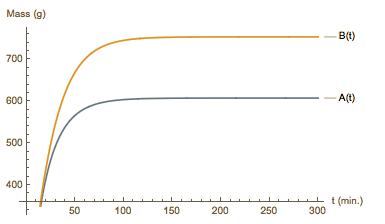
\includegraphics[height=3cm,width=8cm]{W11_WQ_Q10} 
				\end{figure}

					
					\item ``Is there an equilibrium solution to the system?" Correct: $\implies$ \textbf{Yes}
					
					\item ``If so, what is the equilibrium solution?" Correct: $\implies$ \textbf{$\mathbf{\left(\frac{7900}{13},\frac{9800}{13}\right)}$}
				\end{enumerate}
	\end{enumerate}

\end{document}